
\begin{problem}[Question:]{Longest Increasing Subarray | Kadan's Algorithm}
    You are given a array of number, find the longest \textbf{subarray} whose sum is maximum.

    \footnotetext{Pratice Link: \href{https://leetcode.com/problems/maximum-subarray/}{LC53}}
    \footnotetext{Solution File: ./resources/subarray-sum.cpp}
\end{problem}

\begin{solution}[Non Recursive DP]
    \rfl{For all subarray problem, please note that iterative solution is the most natural choise.}
    This is same as for all \underline{subsequence} and \underline{subsequence count problem},recursion is the most natural choice.

    \medskip
    \intution{Let $dp[idx,\_]$ be the the maximum subarray sum, that ends at idx \& \textbf{contains idx}.
    Lets try to write up dp[idx] in terms of subproblem.}
    \footnote{i.e assume that we already know the subproblem answer, now just express dp[idx] in terms of subproblems.}
    
    \medskip
    At dp[idx], we have two choices:
    \begin{asparaenum}[(a)]
        \item \indent Continue the previous subarray. $(val_1 = dp[idx-1]+arr[idx])$
        \item Start a new subarray. $(val_2 = arr[idx])$
    \end{asparaenum}

    \begin{marginfigure}
        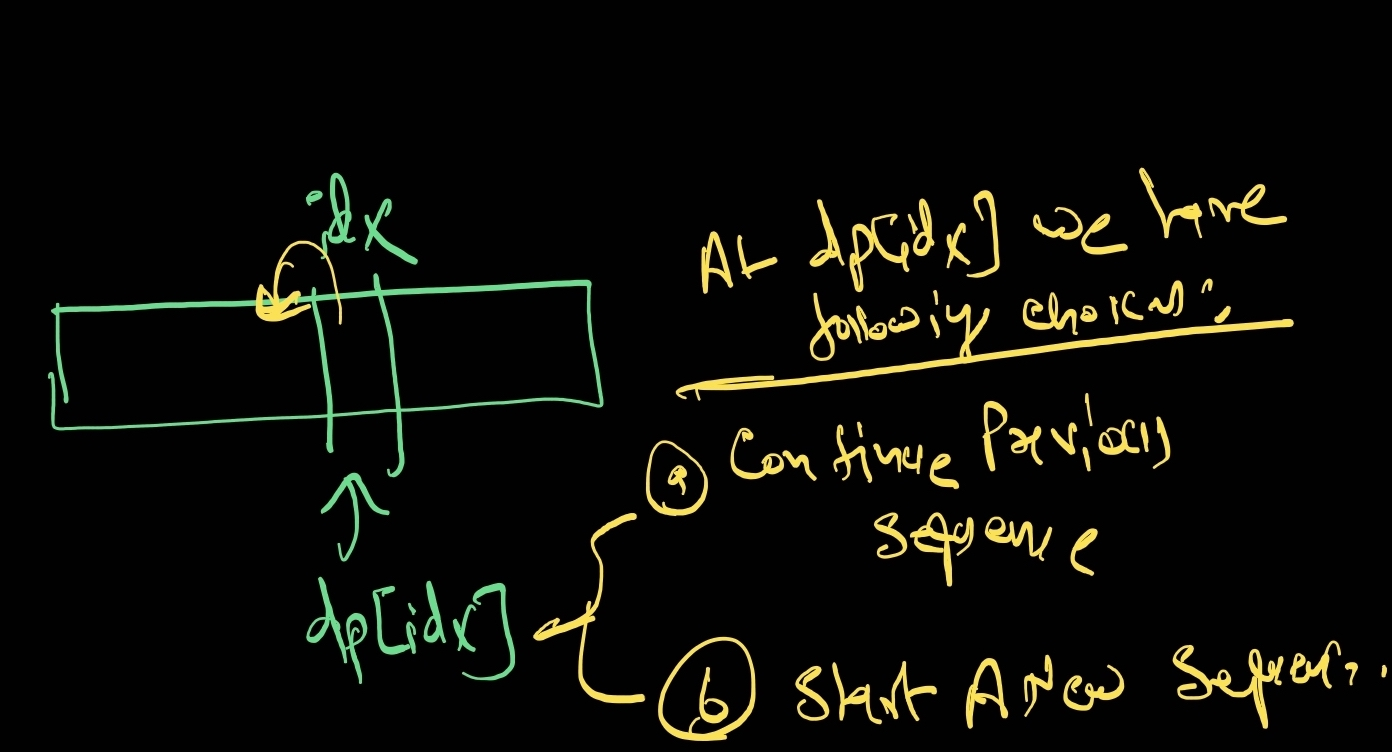
\includegraphics[width=\marginparwidth]{./resources/KadansChoices.jpg}
    \end{marginfigure}

    \medskip
    Hence, for idx we take the best of both $dp[idx] = max(val_1,val_2)$. \\[2mm]
    Now,as we got the maximum subarray when the arr[idx] must be included in the end point of subarray. Our answer be the the maximum amoung all dp[idx].

    \begin{verbatim}
        int maxSubArray(vector<int>& arr) 
        {
            
            int size = arr.size();
            vector<int> dp(arr);
            
            for(int idx=1;idx<size;idx++)
            {
                dp[idx] = max(arr[idx]+dp[idx-1], arr[idx]);
            }

            return *max_element(dp.begin(),dp.end());
    
        }
    \end{verbatim}

\end{solution}

\begin{solution}[Recursive | (Imp) Past State Decision Making]
    Can you build up a solution which usages inclusive/exclusion of subsequence to solve this problem?
    Example: at index idx we have option to continue current sequence OR do not continue.
    TO-DO: can you find the solution?

    % \medskip
    \marginnote{
    This falls under above medium level recursion problem, in which past state is used in current decision making. Up till now, for all question we have the option to either take or not take the element.

    But, \textbf{now this will also be also be restricted based on past state.} accordingly some of the operations will be allowed and some will not.}

    \intution{Let $f(idx,pstate,\_)$ := maximum subarray sum if we are allowed to use arr[idx,size-1]}

    Now at idx, we have the option to \\
    (a) include idx\\
    (b) Do not include idx (Restriction: only if pstate == 0)

    Observe that \rfl{pstate is previous state and not the state at idx.}\\
    - $pstate==0 \implies$ previous element was not selected\\
    - $pstate==1 \implies$ previous element was selected


    \begin{minipage}{\textwidth}
    \begin{lstlisting}
/* f(idx,_) := maximum subarray length when you are allowed to use array arr[idx...last]. Here arr[idx] use is not compulsury.*/
int findAns(int idx,int pstate,vector<int>&arr)
{
    if(idx>= arr.size() ) return pstate == 0? INT_MIN : 0; 

    int &mans = mem[idx][pstate];
    if(mans != -1) return mans;
    
    /* at each idx we have two option */
    int val1=INT_MIN; //include the element 
    int val2=INT_MIN; //do not include the element. (only possible if we have previously not included it)

    if(pstate == 0)
        val2 = findAns(idx+1,0,arr);
    
    // include the arr[idx] & MUST extend to right
    val1 = arr[idx] + findAns(idx+1,1,arr); 

    //include the arr[idx] & NOT extend to right = val11= arr[idx]
    // if f(idx+1) is -ve, then no need to extend to right
    val1 = max(arr[idx],val1); //or val1 = max(val1,val11);

cc  printf("[%d,%d]: (%d,%d)\n",idx,pstate,val1,val2);
    return mans = max({val1,val2});
}

/* pstate for 1st call is zero ,as there was no element to be selected*/
//ans = findAns(0,0,arr); 

\end{lstlisting}
\end{minipage}



\begin{minipage}{\textwidth}
    \rfl{Pratice Problem2: LC2771 Solution, which is subarray problem.}
\begin{lstlisting}

    /* state=0 := no previous element was selected, state=1:= previous element was selected from A, state=2:= previous element was selected from B*/

    /* pstate = previous state & NOT the current state, VERY important to make this observation*/
    int findAnsFive(int idx,int pstate,vector<int>& A, vector<int>& B) 
    {
        if(idx >= A.size()) return 0;
        
        int &mans = mem[idx][pstate];
        if(mans != -1) return mans;
        
        /* at this time we have three options:
            (a) take from A
            (b) take from B
            (c) do not take (for subsequence this is always valid: but for subarray, this is only valid if we MUST HAVE  NOT PICKED any element previously)
        */
        /* Imp for subset sum, we was having two options: take from array , do not array*/
        
        int val1 = 0,val2=0,val3=0;
        
        int pelement = (pstate == 0) ? -1 :((pstate==1) ? A[idx-1]:B[idx-1]);
        
         if(pstate == 0) /* for subarray we can skip taking current element only if we have not taken any previous element*/
            val3 = findAnsFive(idx+1,0,A,B);
        
        if(pelement <= A[idx])
            val1 = 1 + findAnsFive(idx+1,1,A,B);
        if(pelement <= B[idx])
            val2 = 1 + findAnsFive(idx+1,2,A,B);
        
        return mans = max({val1,val2,val3});
    }
\end{lstlisting}
\end{minipage}
\end{solution}

\begin{solution}[Recursion | Follow-Up| Similar Questions]
    Follow Up Question on State Base Recursion Solution.
    \begin{asparaenum}[(a)]
        \item Using above solution, can you first devise recursive kadan's similar solution? 
        Hints: see file /resources/RecursiveToIterativeKadans.cpp
        \item What is the relation between above and LC2771.
        \item Removal of val2 requires us to compute a global maxima, explain what if f(idx) if we do not use val2.
        \item Solve below problems using state based recursion:
        \item LC2771 (recursion+iteration)
        \item LC246 : as subsequence is required and not subarray. hence complexity be O(n*n) instead of O(n*2). (you need to maintain last taken pair)
        \item LC354 Russian Doll Envelopes. This problem ask for just the lenght of the subsequence. Recall that their exist a $O(n*log(n))$ algorithm that can give you longest increasing subsequence length.
    \end{asparaenum}  
\end{solution}

\begin{solution}[Recursive: subarray start at idx | $O(n)$]
    let 
    \intution{$f(idx,\_):=$maximum subarray that starts at idx \& MUST include idx.}

    At each index, we have two option. 
    \begin{asparaenum}[(a)]
        \item Extend the subarray dp[idx+1] at left \textbf{AND start at idx}.
        \item Do not extend the subarray dp[idx+1]. (ie. start a new subarray )
    \end{asparaenum}

    
    \begin{code}
        /* we will calculate dp[idx], where
        dp[idx]:= maximum subarray that starts at idx & MUST include idx.
        i.e idx is the starting point of the sequence*/
        int findAnsTwo(int idx,vector<int>& arr)
        {
            if(idx >= arr.size()) return 0; //no array => 0 sum
            
            if(mem[idx] != INVALID)
                return mem[idx];
            
            /* both start at arr[idx]*/
            int val1; // use dp[idx+1] to extend the subarray on left side
            int val2; //do not use dp[idx+1] to extend the subarray
            
            val1 = arr[idx] + findAnsTwo(idx+1,arr);
            val2 = arr[idx];
            
            return mem[idx] = max(val1,val2);
        }
    \end{code}

    Another way to look at this is that, we want to generate f(idx).
    Since arr[idx] must be included $\implies$ at idx we have only one option to include this element.

    \begin{code}
    //Code File: lisa-RecursiveToIterativeKadans.cpp
        /* sequence start at idx & must include idx*/ /* need to scan for gmx*/
        /* val2 removal requires us to find gmx amoung all answer. */
        int findAnsTwo(int idx,vector<int>&arr)
        {
    
            if(idx>= arr.size() ) return  0; 
       
            int &mans = mem[idx][0];
            if(mans != -1) return mans;
            
/* considerating that we have solution of idx+1.
    At idx we have follwing option
    (a) start a subarray from this point & extend for f(idx+1,arr) (if we consider 
    left to right) OR extend the subarray from dp[idx+1] on left side by including 
    the current element(if we consider how we are processing the recursion result) <= whatever 
    way we consider the end result is same.
*/
            int val1=INT_MIN; //subarray length that start at idx
    
            val1 = arr[idx] + findAns(idx+1,1,arr);
            val1 = max(arr[idx],val1);
            
            gmx = max({gmx,val1});
        cc  printf("[%d]: (%d)\n",idx,val1);
            return mans = val1;
        }
    \end{code}
\end{solution}

\begin{solution}[Recursive: subarray end at idx | $O(n)$]
    Although solving subarray problem in recursive way makes the solution complex.
    Nonetheless, if you want to know how to solve it here is the code.\\[2mm]

    \rfl{
    For subsequence problem, we have recurrance relations as $f(idx)$ := optimal answer for range [0...idx]
    but as this is subarray problem, our $f(idx,_)$ SHOULD be valid only for arr[i...j]}.

    \medskip
    For subarray problem,the defination of recurrance relation changes as \\ \intution{$f(idx,\_)$:= maximum subarray length that ends at idx \& MUST include idx} 
    \medskip

    With above defination of f, at each index idx, we have following options:

    \begin{asparaenum}[(a)]
        \item extends the subarray dp[idx-1] at right \textbf{AND end at idx}.
        \item do not extend the subarray \textbf{and end at idx}.
    \end{asparaenum}

    \begin{code}
        /* we will calculate dp[idx], which is .
        dp[idx] := maximum subarray lenght that ends at idx & MUST include idx*/
        int findAns(int idx,vector<int>& arr)
        {
            if(idx<0) return 0;
            
            if(mem[idx] != INVALID)
                return mem[idx];
            
            int val1 = arr[idx] + findAns(idx-1,arr); //include idx + extend
            int val2 = arr[idx]; //include idx + do NOT extend
            
          cc  printf("[%d]: (%d,%d)\n",idx,val1,val2);
            
            return mem[idx] = max({val1,val2});
            
        }
    \end{code}
\end{solution}




    

\begin{solution}[Divide and Conquer |  $O(n*log(n))$]
    Split the problem in two parts AND build the solution by combing these part.
    
    \begin{code}
    /* this is divide & conquere*/
    int findAnsFour(vector<int>& A, int L, int R){
        if(L > R) return INT_MIN;
        int mid = (L + R) / 2, leftSum = 0, rightSum = 0;

        // leftSum = max subarray sum in [L, mid-1] and starting from mid-1
        for(int i = mid-1, curSum = 0; i >= L; i--)
            curSum += A[i],
        
        leftSum=max(leftSum, curSum);

        // rightSum = max subarray sum in [mid+1, R] and starting from mid+1
        for(int i = mid+1, curSum = 0; i <= R; i++)
            curSum += A[i],
        
        rightSum = max(rightSum, curSum);        

        // return max of 3 cases 
        return max({ findAnsFour(A, L, mid-1), findAnsFour(A, mid+1, R), leftSum + A[mid] + rightSum });
    }	
    \end{code}
\end{solution}


Similary Question List:
\begin{asparaenum}[(a)]
    \item LCXY
\end{asparaenum}